\chapter{Element Parameter Groups}
\label{c:ele.groups}

Generally, element parameters are grouped into ``\vn{element} \vn{parameter} \vn{group}'' 
types. How these groups are used in a lattice element is discussed in \sref{c:ele}. 
This chapter discusses the groups in detail.

The parmeter groups are:
\begin{table}[htb]
\centering
{\tt
\begin{tabular}{llll} \toprule
  {\it Group}        & {\it Section}             & {\it Group}         & {\it Section}         \\ \midrule
 AlignmentGroup      & \sref{s:align.g}          & LordSlaveGroup      & \sref{s:lord.slave.g} \\
 ApertureGroup       & \sref{s:aperture.g}       & MasterGroup         & \sref{s:master.g}     \\
 BMultipoleGroup     & \sref{s:bmultipole.g}     & PatchGroup          & \sref{s:patch.g}      \\ 
 BeamBeamGroup       & \sref{s:beam.beam.g}      & RFCommonGroup       & \sref{s:rfcommon.g}   \\
 BendGroup           & \sref{s:bend.g}           & RFCavityGroup       & \sref{s:rfcavity.g}    \\ 
 EMultipoleGroup     & \sref{s:emultipole.g}     & RFAutoGroup         & \sref{s:rfauto.g}   \\
 FloorPositionGroup  & \sref{s:floor.pos.g}      & ReferenceGroup      & \sref{s:reference.g}  \\
 GirderGroup         & \sref{s:girder.g}         & SolenoidGroup       & \sref{s:solenoid.g}   \\
 InitParticleGroup   & \sref{s:init.particle.g}  & StringGroup         & \sref{s:string.g}     \\
 LCavityGroup        & \sref{s:lcavity.g}        & TrackingGroup       & \sref{s:tracking.g}   \\
 LengthGroup         & \sref{s:length.g}         & TwissGroup          & \sref{s:twiss.g}      \\ 
  \bottomrule
\end{tabular}
} 
\caption{Table of element parameter groups.}
\label{t:particle.groups}
\end{table}

\newpage

%---------------------------------------------------------------------------------------------------

Element parameter groups inherit from the abstract type \vn{EleParameterGroup} which
in turn inherits from \vn{BaseEleParameterGroup}. Some
parameter groups have sub-group components. 
These sub-groups also inherit from \vn{BaseEleParameterGroup}:
\begin{example}
  abstract type BaseEleParameterGroup end
  abstract type EleParameterGroup <: BaseEleParameterGroup end
  abstract type EleParameterSubGroup <: BaseEleParameterGroup end
\end{example}

To see which element types contain a given group, use the \vn{info(::EleParameterGroup)}
method. Example:
\begin{example}
  julia> info(AlignmentGroup)
  ApertureGroup: Vacuum chamber aperture.
  ...
  Found in:
    ACKicker
    Bend
    Kicker
    ...
\end{example}

Notes:
\begin{itemize}
%
\item
All parameter groups have associated docstrings that can be accessed using the REPL help system.
%
\item
NaN denotes a real parameter that is not set.
%
\item
Parameters marked ``dependent'' are parameters calculated by \accellat and not settable by the User.
%
\item
There are several lattice element parameters that are not stored in a parameter group but are stored
alongside of the parameter groups in the element Dict. Included is the element's name, and information
on lords and slaves of the element.
%
\end{itemize}

\newpage

%---------------------------------------------------------------------------------------------------
\section{AlignmentGroup}
\label{s:align.g}

\begin{figure}[bt]
\centering 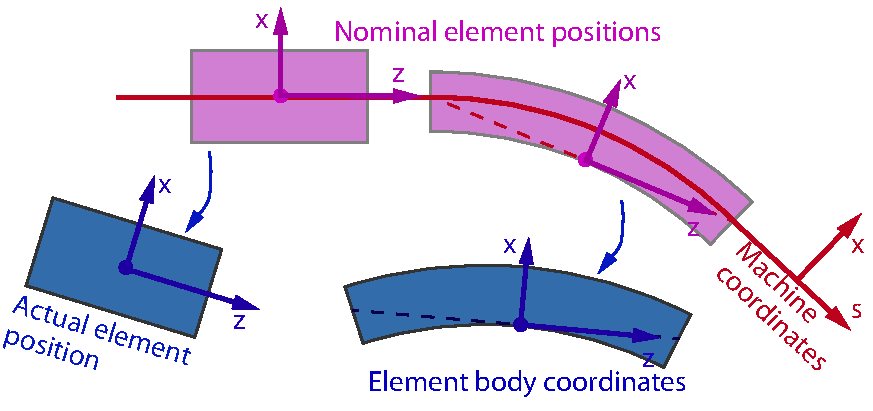
\includegraphics{alignment-ref.pdf} 
\caption[Element alignment.]  
{AlignmentGroup parameters The reference point is the origin
about which the element alignment is calculated. 
A) For straight elements, the reference point is in the center of the element. 
For \vn{Bend} elements, the reference point is at the midpoint of the chord connecting
the entrance point to the exit point. The drawing for the bend is valid for a \vn{ref_tilt}
of zero. For non-zero \vn{ref_tilt}, the outward direction from the bend center will not be
the $x$-axis. 
}  \label{f:alignment}
\end{figure}

\begin{figure}
\centering 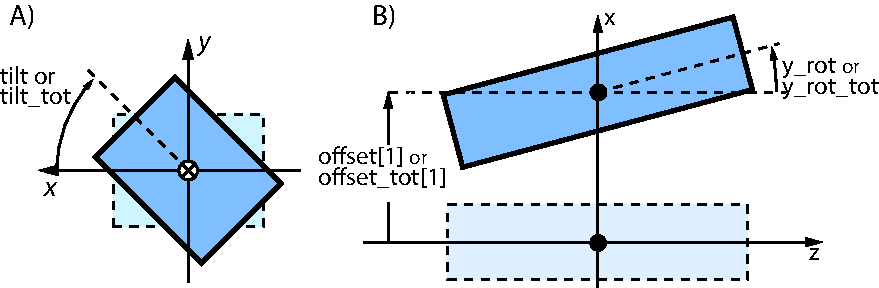
\includegraphics{alignment2.pdf} \caption[Alignment geometry.]  
{Alignment geometry. A) \vn{tilt} (or \vn{tilt_tot}) rotation. B) Combined
\vn{offset[1]} with \vn{y_rot} (or \vn{offset_tot[1]} with \vn{y_rot_tot}).
}  \label{f:alignment}
\end{figure}

The \vn{AlignmentGroup} gives the alignment (position and angular orientation) of the physical element 
relative to the nominal position defined by the machine coordinates (\sref{s:orient}).
Alignment is specified with respect to the ``alignment reference point'' of an element as shown
in Fig~\ref{s:alignment}. The \vn{Bend} reference point is chosen to be the center of the chord
connecting the two ends. 
This reference point was chosen over using the midpoint on the reference orbit arc since a 
common simulation problem is to simulate a bend with a \vn{tilt} keeping the entrance and exit
endpoints fixed.

The parameters of the \vn{AlignmentGroup} can be divided into two sub-groups. 
One group has a \vn{_tot} suffix:
\begin{example}
  offset_tot::Vector - $[x, y, z]$ offset.
  x_rot_tot::Number  - Rotation around the x-axis.
  y_rot_tot::Number  - Rotation around the z-axis.
  tilt_tot::Number   - Rotation around the z-axis. 
\end{example}
These ``total alignment'' parameters give the alignment of the element with 
with respect to the machine coordinates.
The other sub-group of parameters do not have a \vn{_tot} suffix:
\begin{example}
  offset::Vector - $[x, y, z]$ offset.
  x_rot::Number  - Rotation around the x-axis.
  y_rot::Number  - Rotation around the z-axis.
  tilt::Number   - Rotation around the z-axis. 
\end{example}
These ``relative alignment'' parameters give the alignment of the element with respect 
to any \vn{Girder} that is supporting the element. 
If there is no support \vn{Girder}, the total alignment will be the same as the relative
alignment. The relative alignment can be set by the User. 
The total alignment is computed by \accellat based upon the relative alignment and the alignment
of any \vn{Girder}. \vn{Girder} elements themselves also have both relative and total
alignments since Girders can support other Girders.

\newpage

%---------------------------------------------------------------------------------------------------
\section{ApertureGroup}
\label{s:aperture.g}

\begin{figure}[bt]
\centering 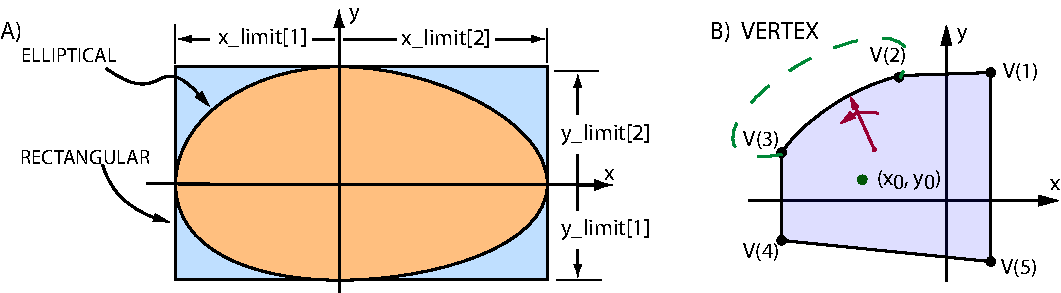
\includegraphics{apertures.pdf} \caption[Rectangular and elliptical apertures.]  
{
Rectangular and elliptical apertures. As drawn, \vn{x_limit[1]} and \vn{y_limit[1]} are 
negative and \vn{x_limit[2]} and \vn{y_limit[2]} are positive.
}  \label{f:aperture}
\end{figure}

The \vn{ApertureGroup} stores information about apertures an element may have. 
The parameters of this group are:
\begin{example}
  x_limit::Vector{Number}                     - 2-Vector of horizontal aperture limits. (m)  
  y_limit::Vector{Number}                     - 2-Vector of vertical aperture limits. (m)  
  vertex::Vector{AcceleratorLattice.Vertex1}  - Array of aperture vertexes. ()  
  aperture_shape::ApertureShape               - Shape of aperture. Default is ELLIPTICAL. ()  
  aperture_at::AcceleratorLattice.BodyLoc.T   - Where the aperture is. Default is BodyLoc.ENTRANCE_END. ()  
  misalignment_moves_aperture::Bool           - Does moving the element move the aperture? ()  
\end{example}

The aperture location of 

%---------------------------------------------------------------------------------------------------
\section{BMultipoleGroup}
\label{s:bmultipole.g}

%---------------------------------------------------------------------------------------------------
\section{BeamBeamGroup}
\label{s:beam.beam.g}

%---------------------------------------------------------------------------------------------------
\section{BendGroup}
\label{s:bend.g}

The \vn{BendGroup} stores the parameters that characterize the shape of a \vn{Bend} element
\sref{s:bend}. The only relavent shape parameter that is not in the \vn{BendGroup} is the
length \vn{L} which is in the \vn{LengthGroup}.

The parameters of this group are:

\begin{figure}[ht]
  \centering 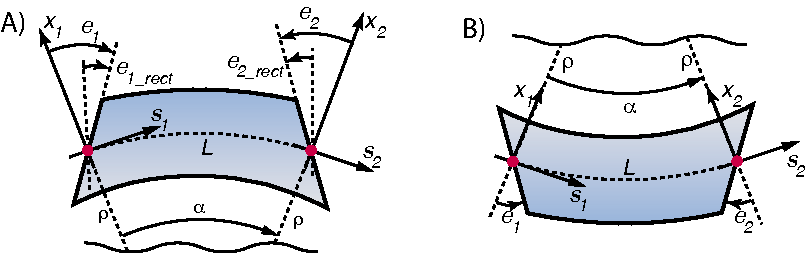
\includegraphics{bend.pdf} 
\caption[Bend geometry]{
Bend geometry. Red dots are the entry and exit points that define the origin for the
coordinate systems at the entry end $(s_1, x_1)$ and exit ends $(s_2, x_2)$ respectively. 
In the figure, the angle \vn{alpha} is denoted $\alpha$ and the radius
\vn{rho} is denoted $\rho$.
A) Bend geometry with positive bend angle. For the geometry shown, 
\vn{g}, \vn{angle}, \vn{rho}, \vn{e1}, \vn{e2}, \vn{e1_rect}, and \vn{e2_rect} are all positive.
B) Bend geometry with negative bend angle. For the geometry shown, 
\vn{g}, \vn{angle}, \vn{rho}, \vn{e1}, \vn{e2}, \vn{e1_rect}, and \vn{e2_rect} are all negative.
Note: The figures are drawn for zero \vn{ref_tilt} where the rotation axis is parallel to the 
$y$-axis. 
}
\label{f:bend}
\end{figure}

\vn{BendGroup} parameters are:
  \begin{description}
  %
  \index{angle}
  \item[angle] \Newline
The total design bend angle. A positive \vn{angle} represents a
bend towards negative $x$ as shown in \fig{f:bend}.
  %
  \index{bend_field}
  \item[bend_field] \Newline
The \vn{bend_field} parameter is the design magnetic bending field which determines the reference orbit
and the placement of lattice elements downstream from the bend. The actual (``total'') field is
a vector sum of
\vn{bend_field} plus the value of the \vn{Bn0}  and \vn{Bs0} multipoles. If \vn{tilt0} and \vn{Bs0}
are zero, the actual field is
\begin{example}
  B-field (total) = bend_field + Bn0
\end{example}
See the discussion of \vn{g} and \vn{Kn0} below for more details.
  %
  \item[bend_type] \Newline
The \vn{bend_type} parameter sets the ``logical shape'' of the bend. 
This parameter is of type \vn{BendType.T} (\sref{s:bendtype}) and can take values of
\begin{example}
  BendType.RECTANGULAR  - or
  BendType.SECTOR       - The default
\end{example}
The logical shape of a bend, in most situations, is irrelevant. 
The only case where the logical shape is used is when the bend angle is varied. 
In this case, for a \vn{SECTOR} bend, the face angles \vn{e1} and \vn{e2} are 
held constant and \vn{e1_rect} and \vn{e2_rect} are varied to keep \Eqs{eeaeea} satisfied.
  %
  \index{e1}\index{e2}
  \item[e1, e2] \Newline
The values of \vn{e1} and \vn{e2} gives the rotation angle of the entrance and exit pole faces
respectively with respect to the radial $x_1$ and $x_2$ axes as shown in \fig{f:bend}.
Zero \vn{e1} and \vn{e2} gives a wedge shaped magnet.
Also see \vn{e1_rect} and \vn{e2_rect}. The relationship is
\begin{equation}
  \parbox{30em} {
    e1 = e1_rect + angle/2 \\
    e2 = e2_rect + angle/2
  }
  \label{eeaeea}
\end{equation}

Note: The correspondence between \vn{e1} and \vn{e2} and the corresponding parameters used in the
SAD program \cite{b:sad} is:
\begin{example}
  e1(AccelLat) =  e1(SAD) * angle + ae1(SAD)
  e2(AccelLat) =  e2(SAD) * angle + ae2(SAD)
\end{example}
  %
  \item[e1_rect, e2_rect]
Face angle rotations like \vn{e1} and \vn{e2} except angles are measured with respect to 
fiducial lines that are parallel to each other and rotated by \vn{angle}/2 from the radial
$x_1$ and $x_2$ axes as shown in \fig{f:sbend}. 
Zero \vn{e1_rect} and \vn{e2_rect} gives a rectangular magnet shape.
  %
  \index{exact_multipoles}
  \item[exact_multipoles] \Newline
The \vn{exact_multipoles} switch can be set to one of:
\begin{example}
  off                 ! Default
  vertically_pure    
  horizontally_pure  
\end{example}
This switch determines if the multipole fields, both magnetic and electric, and including the
\vn{k1} and \vn{k2} components, are corrected for the finite curvature of the reference orbit in a
bend. See \sref{s:field.exact} for a discussion of what \vn{vertically} pure versus
\vn{horizontally} pure means. Setting \vn{exact_multipoles} to \vn{vertically_pure} means that the
individual $a_n$ and $b_n$ multipole components are used with the vertically pure solutions
\begin{equation}
  \bfB = \sum_{n = 0}^\infty \left[ \frac{a_n}{n+1} \nabla \phi_n^r + \frac{b_n}{n+1} \nabla \phi_n^i \right], \qquad
  \bfE = \sum_{n = 0}^\infty \left[ \frac{a_{en}}{n+1} \nabla \phi_n^i + \frac{b_{en}}{n+1} \nabla \phi_n^r \right]
\end{equation}
and if \vn{exact_multipoles} is set to \vn{horizontally_pure} the horizontally pure solutions
$\psi_n^r$ and $\psi_n^i$ are used instead of the vertically pure solutions $\phi_n^r$ and
$\phi_n^i$.
  %
  \index{fint1}\index{fint2}\index{hgap1}\index{hgap2}
  \item[fint1, fint2, hgap1, hgap2] \Newline
The field integrals for the entrance pole face is given by the product of the \vn{fint} and
\vn{hgap} parameters with \vn{hgap} being the half gap between poles at the entrance face
\begin{equation}
  F_{H1} \equiv F_{int1} \, H_{gap1} = \int_{pole} \! \! ds \, \frac{B_y(s) \, (B_{y0} - B_y(s))}
  {2 \, B_{y0}^2}
  \label{fsbbb}
\end{equation}
For the exit pole face there is a similar equation using \vn{fint2} and \vn{hgap2} which defines
$F_{H2}$. In the above equation $B_{y0}$ is the field in the interior of the dipole. The values of
\vn{fint1}, \vn{fint2}, \vn{hgap1}, and \vn{hgap2} are never used in isolation when tracking. Only
the values for $F_{H1}$ and $F_{H2}$ matter.
That is, to have an effect, both \vn{fint} and \vn{hgap} (or \vn{fintx} and \vn{hgapx}) must be non-zero.

Note: The SAD program uses \vn{fb1+f1} for the entrance fringe and \vn{fb2+f1} for the exit
fringe. The correspondence between the two is
\begin{example2}
  \(F_{H1}\) = fint  * hgap  = (fb1 + f1) / 12
  \(F_{H2}\) = fintx * hgapx = (fb2 + f1) / 12
\end{example2}

\index{Enge function}
\vn{fint} and \vn{hgap} can be related to the Enge function which is sometimes used to model the
fringe field. The Enge function is of the form
\begin{equation}
  B_y(s) = \frac{B_{y0}}{1 + \exp[P(s)]}
\end{equation}
where
\begin{equation}
  P(s) = C_0 + C_1 \, s + C_2 \, s^2 + C_3 \, s^3 + \, \ldots
\end{equation}
The $C_0$ term simply shifts where the edge of the bend is. If all the $C_n$ are zero except for
$C_0$ and $C_1$ then
\begin{equation}
  C_1 = \frac{1}{2 \,H_{gap} \, F_{int}}
\end{equation}
  %
  \item[fiducial_pt] \Newline
The \vn{fiducial_pt} parameter sets a fiducial point which can be used to keep the shape of the bend
constant when, in a program, the parameters \vn{rho}, \vn{g}, \vn{b_field} or \vn{angle} are varied.
Varying these parameters typically happens when doing machine design. Using a fiducial point can be
helpful when designing a machine usin bend magnets that already exist.

The \vn{fiducial_pt} parameter
has four possible settings:
\begin{example}
  none          ! No fiducial point (default).
  entrance_end  ! The entrance point is the fiducial point.
  center        ! The center of the reference curve is the fiducial point.
  exit_end      ! The exit point is the fiducial point.
\end{example}
With \vn{fiducial_pt} set to \vn{none} (the default). The bend shape is not held constant. With the
other three settings, the bend shape will be held constant as discussed in \sref{s:bend.fiducial}.
With \vn{fiducial_pt} set to \vn{entrance_end}, the reference trajectory at the entrance end is held
fixed in both position and orientation with respect to the bend face and \vn{g}, \vn{l} and \vn{e2},
along with the other depdendent parameters, are adjusted to both give the desired change in what was
varied (which is one of \vn{rho}, \vn{g}, \vn{b_field} or \vn{angle}) and to keep the shape of the
bend unchanged. See \fig{f:bend.fid1}. Similarly, if \vn{fiducial_pt} is set to \vn{center}, the
center of the reference trajectory is held fixed in both position and orientation and if
\vn{fiducial_pt} is set to \vn{exit_end}, the exit point is held fixed in both position and
orientation.
  %
  \index{g}\index{rho}
  \item[g, rho] \Newline
The design bending radius which determines the reference coordinate system is \vn{rho} (see
\sref{s:ref}). \vn{g} = \vn{1/rho} is the ``bend strength'' and is proportional to the design
dipole magnetic field. \vn{g} is related to the design magnetic field \vn{bend_field} via
\begin{equation}
  \text{g} = \frac{q}{p_0} \, \text{bend_field} 
  \label{gqpb}
\end{equation}
where $q$ is the charge of the reference particle and $p_0$ is the reference momentum. It is
important to keep in mind that changing \vn{g} will change the design orbit (\sref{s:coords.3}) and
hence will move all downstream lattice elements in space.

The total bend strength felt by a particle is the vector sum of \vn{g} plus the zeroth order
magnetic multipole. If the multipole \vn{tilt0} and \vn{Ks0} is zero, the total bend strength is
\begin{example}
  g_total = g + Kn0
\end{example}
Changing the multipole strength \vn{Kn0} or \vn{Ks0} leaves the design orbit and the positions of
all downstream lattice elements
unchanged but will vary a particle's orbit. One common mistake when designing lattices is to vary
\vn{g} and not \vn{Kn0} which results in downstream elements moving around. See \Sref{s:ex.chicane}
for an example.

Note: A positive \vn{g}, which will bend particles and the reference orbit in the $-x$ direction
represents a field of opposite sign as the field due a positive \vn{hkick}.
  %
  \index{h1}\index{h2}
  \item[h1, h2] \Newline
The attributes \vn{h1} and \vn{h2} are the curvature of the entrance and exit pole faces.
  %
  \index{L}\index{L_chord}\index{L_arc}\index{L_sagitta}
  \item[L, L_arc, L_chord, L_sagitta]  \Newline
The \vn{L} parameter, which is in the \vn{LengthGroup} and not the \vn{BendGroup}, 
is the arc length of the reference trajectory through the bend.

\vn{L_chord} is the chord length from entrance point to exit point.
The \vn{L_sagitta} parameter is the sagitta length (The sagitta is the distance
from the midpoint of the arc to the midpoint of the chord). \vn{L_sagitta} can be negative and will have
the same sign as the \vn{g} parameter.
  %
  \item[L_rectangle] \Newline
The \vn{L_rectangle} parameter is the ``rectangular'' length defined to be the distance between the
entrance and exit points. The coordinate system used for the calculation is defined by the setting
of \vn{fiducial_pt}. \fig{f:rbend} shows \vn{l_rectangle} for \vn{fiducial_pt} set to
\vn{entrance_end} (the coordinate system corresponds to the entrance coordinate system of the bend).
In this case, and in the case where \vn{fiducial_pt} is set to \vn{exit_end}, the rectangular
length will be $\rho \sin\alpha$. If \vn{fiducial_pt} is set to \vn{none} or \vn{center},
\vn{l_rectangle} is the same as the chord length.
  %
  \index{ref_tilt}
  \item[ref_tilt] \Newline
The \vn{ref_tilt} attribute rotates a bend about the longitudinal axis at the entrance face of the
bend. A bend with \vn{ref_tilt} of $\pi/2$ and positive \vn{g} bends the element in the $-y$
direction (``downward''). See \fig{f:tilt.bend}. It is important to understand that \vn{ref_tilt},
unlike the \vn{tilt} attribute of other elements, bends both the reference orbit along with the
physical element. Note that the MAD \vn{tilt} attribute for bends is equivalent to the \bmad
\vn{ref_tilt}. Bends in \bmad do not have a \vn{tilt} attribute.

Important! Do not use \vn{ref_tilt} when doing misalignment studies for a machine. Trying to misalign
a dipole by setting \vn{ref_tilt} will affect the positions of all downstream elements! Rather, use the
\vn{tilt} parameter.
  \end{description}

%---------------

The attributes \vn{g}, \vn{angle}, and \vn{L} are mutually dependent. If any two are specified for
an element \bmad will calculate the appropriate value for the third.

In the local coordinate system (\sref{s:ref}), looking from ``above'' (bend viewed from positive
$y$), and with \vn{ref_tilt} = 0, a positive \vn{angle} represents a particle rotating clockwise. In
this case. \vn{g} will also be positive. For counterclockwise rotation, both \vn{angle} and \vn{g}
will be negative but the length \vn{l} is always positive. Also, looking from above, a positive
\vn{e1} represents a clockwise rotation of the entrance face and a positive \vn{e2} represents a
counterclockwise rotation of the exit face. This is true irregardless of the sign of \vn{angle} and
\vn{g}. Also it is always the case that the pole faces will be parallel when
\begin{example}
  e1 + e2 = angle
\end{example}

%---------------------------------------------------------------------------------------------------
\section{EMultipoleGroup}
\label{s:emultipole.g}

%---------------------------------------------------------------------------------------------------
\section{FloorPositionGroup}
\label{s:floor.pos.g}

%---------------------------------------------------------------------------------------------------
\section{GirderGroup}
\label{s:girder.g}

%---------------------------------------------------------------------------------------------------
\section{InitParticleGroup}
\label{s:init.particle.g}

%---------------------------------------------------------------------------------------------------
\section{LCavityGroup}
\label{s:lcavity.g}

%---------------------------------------------------------------------------------------------------
\section{LengthGroup}
\label{s:length.g}

%---------------------------------------------------------------------------------------------------
\section{LordSlaveGroup}
\label{s:lord.slave.g}

%---------------------------------------------------------------------------------------------------
\section{MasterGroup}
\label{s:master.g}

%---------------------------------------------------------------------------------------------------
\section{PatchGroup}
\label{s:patch.g}

%---------------------------------------------------------------------------------------------------
\section{RFCommonGroup}
\label{s:rfcommon.g}

%---------------------------------------------------------------------------------------------------
\section{RFCavityGroup}
\label{s:rfcavity.g}

%---------------------------------------------------------------------------------------------------
\section{RFAutoGroup}
\label{s:rfauto.g}

%---------------------------------------------------------------------------------------------------
\section{ReferenceGroup}
\label{s:reference.g}

%---------------------------------------------------------------------------------------------------
\section{SolenoidGroup}
\label{s:solenoid.g}

%---------------------------------------------------------------------------------------------------
\section{StringGroup}
\label{s:string.g}

%---------------------------------------------------------------------------------------------------
\section{TrackingGroup}
\label{s:tracking.g}

%---------------------------------------------------------------------------------------------------
\section{TwissGroup}
\label{s:twiss.g}

